\documentclass{lecturenotes}

\title[Kort presentation av PtD \& DoD, 2015-08-27]{\href{http://cs.lth.se/eda016}{EDA016} Programmeringsteknik för D (PtD) \\ + \\ \href{http://cs.lth.se/eda070}{EDA070} Datorer och datoranvändning (DoD)}
\author{\href{http://cs.lth.se/bjorn-regnell}{Björn Regnell}, \href{http://cs.lth.se/roger_henriksson}{Roger Henriksson}}
\institute{\href{http://cs.lth.se}{Datavetenskap}, LTH}
\date{2015-08-27}
 
\begin{document}
 
\frame{\titlepage}

%\SlideImg{Att lägga grunden \href{http://www.vhuset.lth.se/v-husets-bibliotek/om-v-biblioteket/byggandet-av-lth/}{...}}{img/lthgrund.jpg}
%Bilden av grundläggningen av Mattehuset, LTH från juni 1963 

\frame{\frametitle{En kurskombo som startar på måndag kl 13:15 i E:B}
Lägger grunden för alla kommande kurser i datavetenskap: \vspace{1em}
\begin{itemize}
\item Programmeringsteknik för D, 7.5 hp, 16 veckor
\begin{itemize}
\item[] Grundlig genomgång av programmering från början
\end{itemize}
\vspace{1em}
\item Datorer och datoranvändning, 3 hp, 3 veckor
\begin{itemize}
\item[] Inblick i hur datorer fungerar och verktygen vi använder
\end{itemize}
\end{itemize}
}

\frame{\frametitle{Vad ska du lära dig?}
%Att skapa koden som styr världen...
%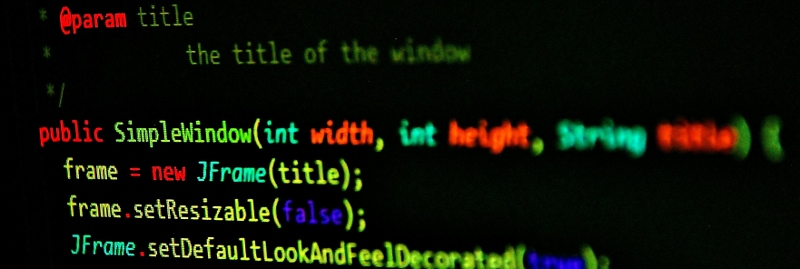
\includegraphics[width=1.2\textwidth, height=1.5cm]{img/code-wide}
\begin{multicols}{2}
\begin{itemize}\Size{9pt}
\item \textbf{Programmeringsteknik för D}
\begin{itemize}\Size{8pt}
\item Programmering från grunden
\item Konstruera algoritmer
\item Tänka i abstraktioner
\item Programspråket Java
\item Utvecklingsmiljön Eclipse
\end{itemize}
\columnbreak
\item \textbf{Datorer \& datoranvändning}
\begin{itemize}\Size{8pt}
\item Lågnivåprogrammering
\item Internet
\item Terminalkommando i Linux
\item Skriva \& typsätta i \LaTeX
\item Beräkningar i Matlab
\end{itemize}
\end{itemize}
\end{multicols}
\flushright\scriptsize Denna presentation i \LaTeX ~på GitHub:\\\url{http://cs.lth.se/eda016/lecturenotes}
}

%%%
\frame{\frametitle{Hur ska du lära dig?}
\begin{itemize}
\item Genom praktiskt eget arbete: Lära genom att göra!
\item Genom studier av kursteorin: Skapa förståelse
\item Genom samarbete med dina kurskamrater
\end{itemize}
}

\SlideImg{Stor spridning i programmeringsförkunskaper\\ bland D-are (enl. enkätsvar 2010-2014)}{img/pre-pie}

%%%
\frame[plain]{\frametitle{Förkunskapsenkät}
\begin{itemize}
\item Har du programmerat innan du kom till LTH? \\
         Ja \hspace{2.5cm} Nej %\hskip8mm\lstinline+if  (svar.equals("Nej")) {break}+
\item Hur många program har du skrivit? \\ 
         $<5$ \hspace{2.2cm} $5-20$ \hspace{2.5cm}  $>20$
\item Hur stort var det största program du har skrivit?\\ 
         $<50$ rader \hspace{1cm} $50 - 500$  rader \hspace{1cm}  $>500$ rader
\end{itemize}
\vspace{1em}
Fyll i denna enkät idag:
\url{http://cs.lth.se/eda016/survey}
}

%%%
\frame{\frametitle{Skaffa kurslitteratur} 
\footnotesize
\begin{columns}
\begin{column}{0.45\textwidth}
EDA016 PtD:
\begin{itemize}
\item \Emph{Bokpaket} säljs på KFS \\John Ericssons väg 4 \url{http://www.kfsab.se/}
\begin{itemize}
\item ''Objektorienterad programmering och Java'' av Per Holm
\item Kurskompendium med övningar och laborationer
\end{itemize}
\end{itemize}
EDA070 DoD:
\begin{itemize}
\item Säljs på första föreläsningen
\item Ta med \Emph{50 kr jämna pengar}
\end{itemize}
\end{column}
\begin{column}{0.5\textwidth}
\centering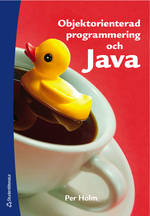
\includegraphics[width=0.7\textwidth]{img/ankbok.jpg}
\end{column}
\end{columns}


}

\SlideImg{Välkommen på måndag kl 13:15 i E:B}{img/ehuset}


\end{document}

